\chapter{مِمَّ تُصنع الأشياء؟}\label{ch:g1:materials-around-us}

انظر إلى مائدة الفطور. عليها ملعقة، وكأس حليب، وشوكة، ومنديل، وصحن
عميق، وكنزة معلقة على ظهر كرسي. أشياء كثيرة، وكل واحد منها مصنوع من
شيء ما: الملعقة من الخشب، والشوكة من المعدن، والكأس من الزجاج،
والمنديل من الورق، والصحن من البلاستيك، والكنزة من الصوف. مائدة مليئة
بالأشياء، وهي مصنوعة من عدد قليل من المواد المختلفة. وعن هذه المواد
يتحدث هذا الفصل.

\begin{omfigure}
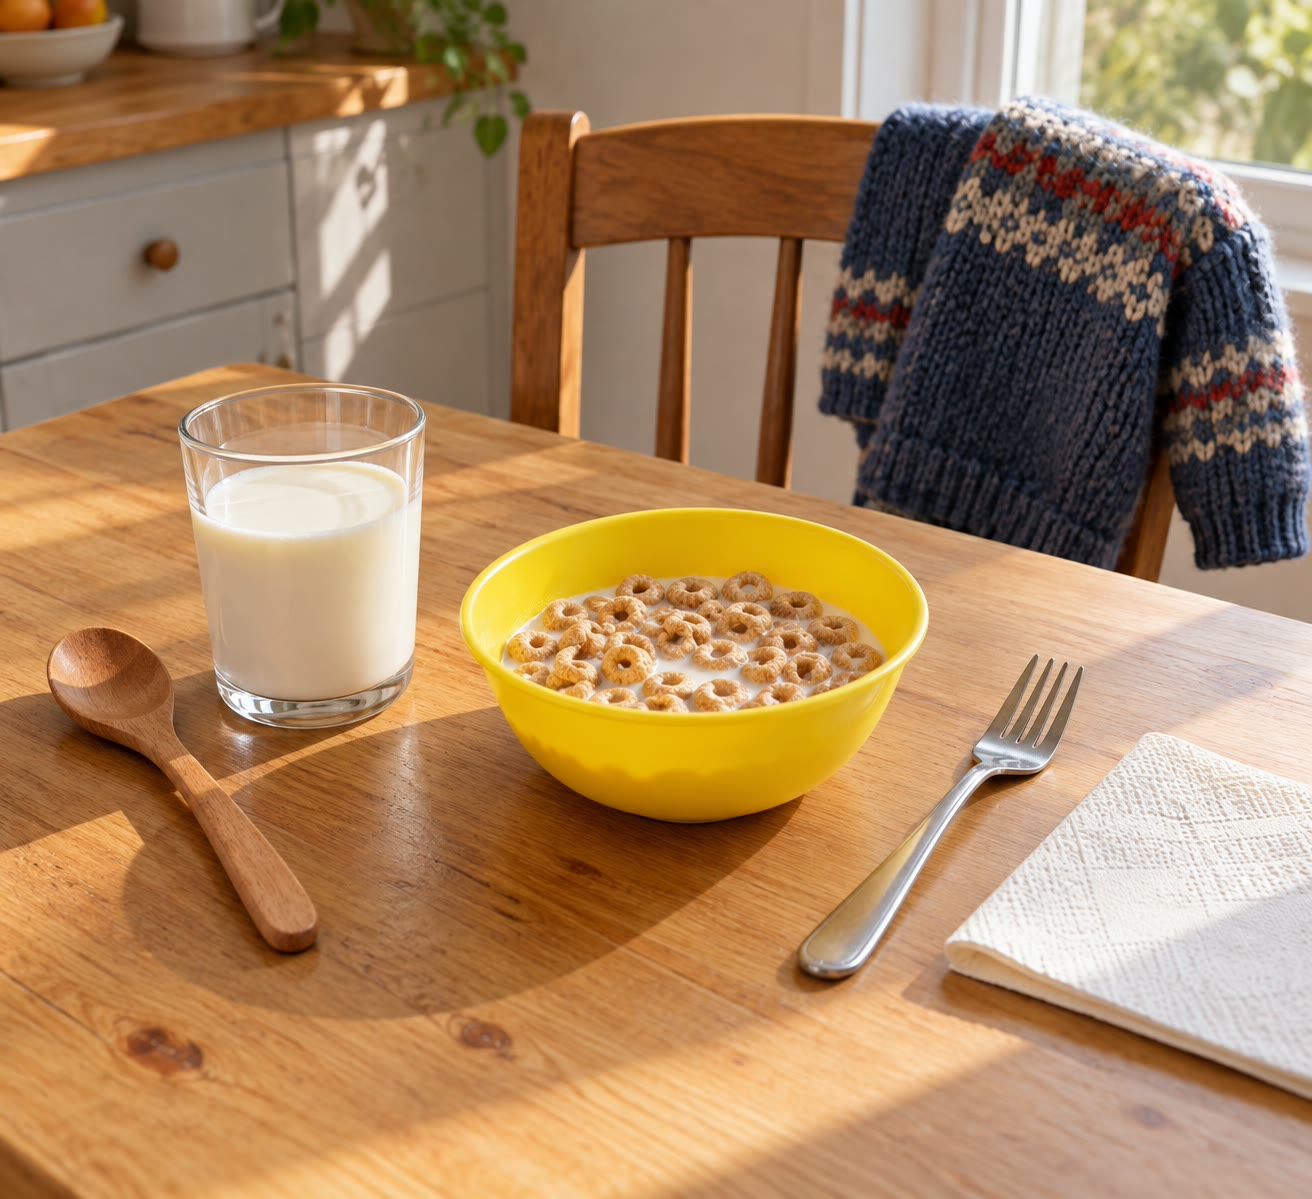
\includegraphics[width=0.62\linewidth]{images/book1/ai/g1-breakfast-table.jpg}

{\small مائدة الفطور: أشياء كثيرة مصنوعة من مواد قليلة.}
\end{omfigure}

\section{الأجسام والمواد}

\begin{definition}[الجسم]\label{def:g1:materials-around-us:object}
\emph{الجسم}\index{جسم} شيء نراه ونلمسه، وكثيرًا ما نمسكه ونستعمله:
ملعقة، أو كرسي، أو كرة، أو نافذة، أو حذاء.
\end{definition}

\begin{definition}[المادة]\label{def:g1:materials-around-us:material}
\emph{مادة}\index{مادة} \omterm{def:g1:materials-around-us:object}{الجسم} هي ما صُنع منه \omterm{def:g1:materials-around-us:object}{الجسم}. قد تُصنع الملعقة
من الخشب أو من المعدن أو من البلاستيك: الملعقة هي \omterm{def:g1:materials-around-us:object}{الجسم}، والخشب هو
المادة.
\end{definition}

\begin{example}[جسم واحد وثلاث مواد]\label{ex:g1:materials-around-us:spoons}
ثلاث ملاعق متجاورة. لها الشكل نفسه وتؤدي العمل نفسه، فهي إذن من النوع
نفسه من الأجسام. لكن واحدة مصنوعة من الخشب، وواحدة من المعدن، وواحدة
من البلاستيك: ثلاث مواد مختلفة.
\end{example}

\begin{omfigure}
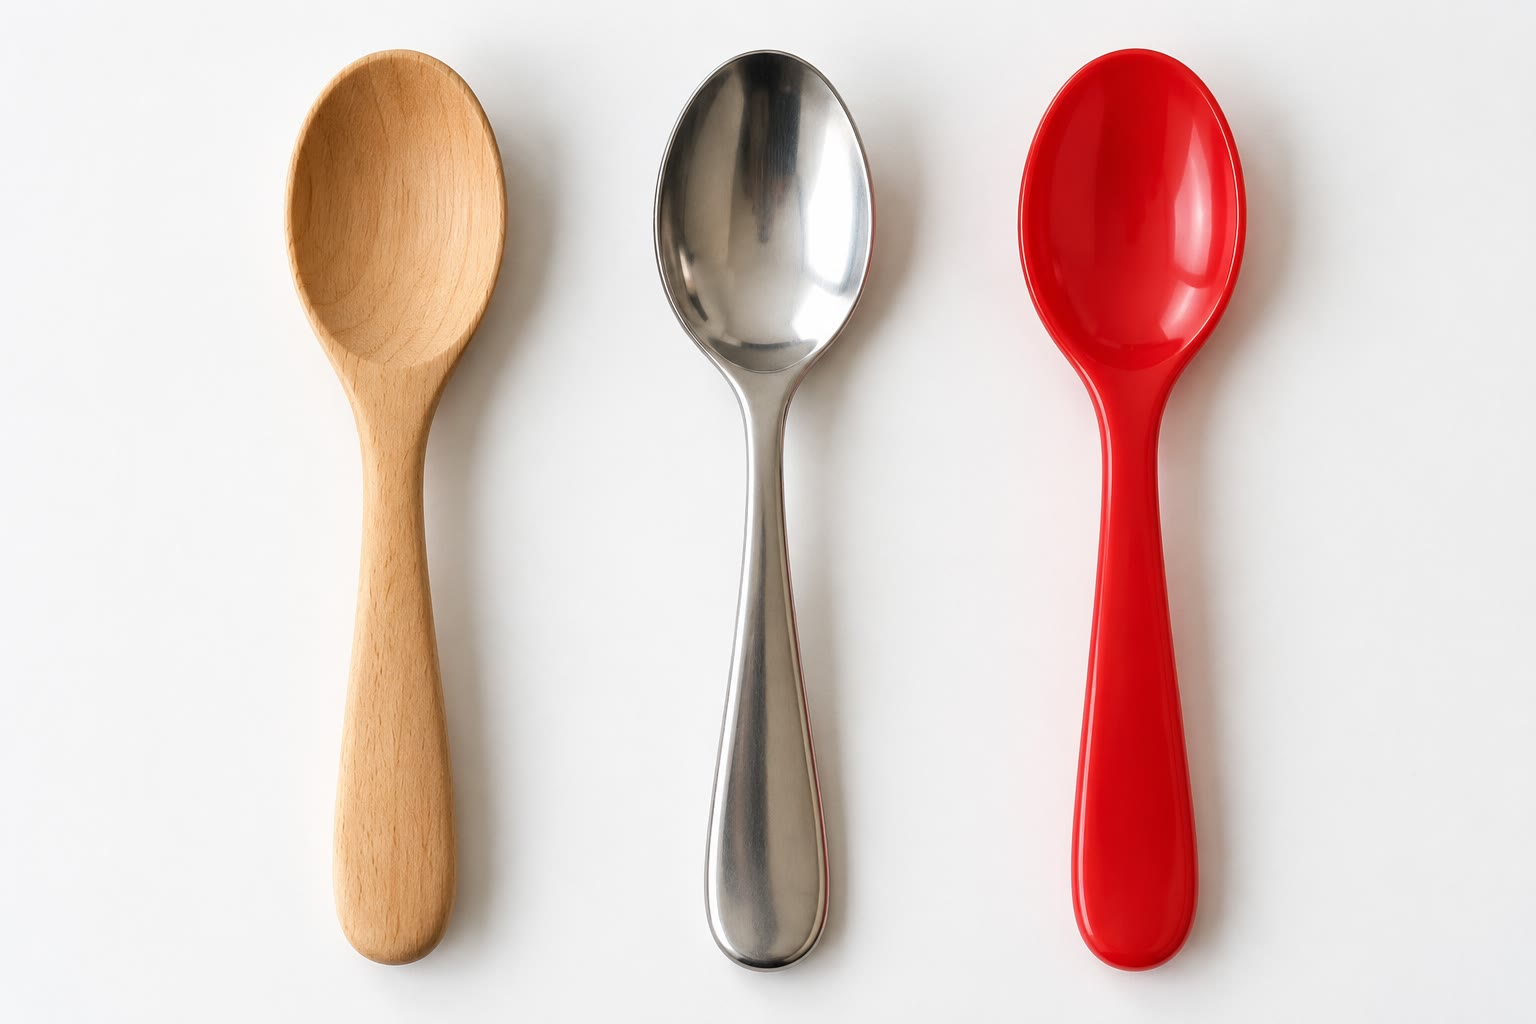
\includegraphics[width=0.55\linewidth]{images/book1/ai/g1-three-spoons.jpg}

{\small ثلاث ملاعق: \omterm{def:g1:materials-around-us:object}{جسم} واحد وثلاث مواد --- الخشب والمعدن
والبلاستيك.}
\end{omfigure}

\begin{example}[مادة واحدة وأجسام كثيرة]\label{ex:g1:materials-around-us:wood}
الخشب \omterm{def:g1:materials-around-us:material}{مادة} قلم الرصاص، والكرسي، والباب، وقطار اللعب، والملعقة
الخشبية. يمكن أن تُصنع أجسام كثيرة مختلفة من \omterm{def:g1:materials-around-us:material}{المادة} نفسها.
\end{example}

\begin{remark}[أجسام من عدة مواد]\label{rem:g1:materials-around-us:several}
كثير من الأجسام مصنوع من أكثر من \omterm{def:g1:materials-around-us:material}{مادة} واحدة. فللمقص شفرتان من المعدن
ومقبضان من البلاستيك. وقلم الرصاص خشب من الخارج وفي داخله عود رمادي
من الغرافيت. والنافذة زجاج في إطار من الخشب أو المعدن أو البلاستيك.
\end{remark}

\section{سبع مواد شائعة}

\begin{proposition}[المواد من حولنا]\label{prop:g1:materials-around-us:seven}
معظم الأجسام من حولنا مصنوعة من مواد قليلة شائعة:
\begin{itemize}
  \item \textbf{الخشب}: الطاولات، والكراسي، وأقلام الرصاص، والأبواب؛
  \item \textbf{المعدن}: الشوكات، والمفاتيح، والمسامير، والقدور، والدراجات؛
  \item \textbf{الزجاج}: النوافذ، والمرطبانات، والقوارير، والكؤوس؛
  \item \textbf{البلاستيك}: الصحون، والقوارير، والألعاب، والدلاء؛
  \item \textbf{الورق} والورق المقوى: الكتب، والمناديل، والعلب؛
  \item \textbf{القماش}: الملابس، والستائر، والحقائب --- وهو مصنوع من الصوف
        أو القطن أو خيوط أخرى؛
  \item \textbf{الحجر}: الجدران، والدرجات، والحصى، والتماثيل.
\end{itemize}
\end{proposition}

\begin{omfigure}
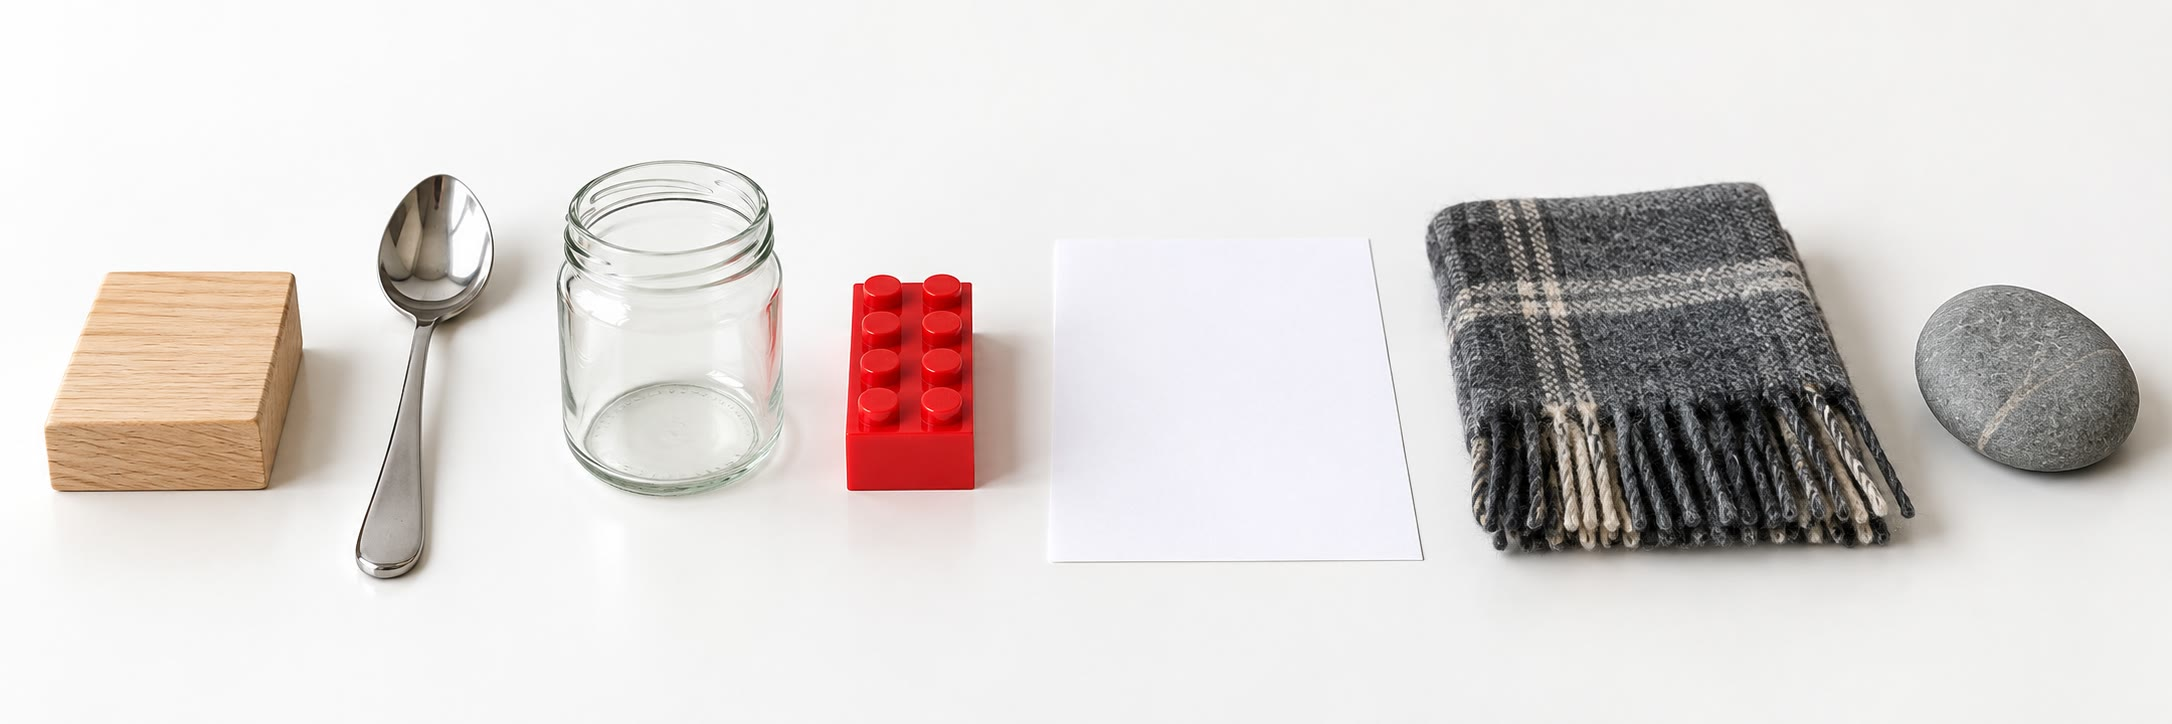
\includegraphics[width=0.75\linewidth]{images/book1/ai/g1-material-samples.jpg}

{\small سبع عينات، من اليسار إلى اليمين: الخشب، والمعدن، والزجاج،
والبلاستيك، والورق، والقماش (الصوف)، والحجر.}
\end{omfigure}

\begin{remark}[أسماء مأخوذة من المواد]\label{rem:g1:materials-around-us:names}
نسمي القارورة «زجاجة» لأنها مصنوعة من الزجاج، ونسمي القطعة من الورق
«ورقة». فاسم \omterm{def:g1:materials-around-us:object}{الجسم} يُشتق هنا من اسم مادته، والكلمتان متقاربتان. وحين
نتحدث عن المواد نقصد ما صُنع منه الشيء، لا الشيء نفسه.
\end{remark}

\section{خصائص المواد}

\begin{definition}[خاصية المادة]\label{def:g1:materials-around-us:property}
\emph{خاصية المادة}\index{خاصية المادة} شيء نعرفه عنها بالنظر أو
اللمس أو الاختبار: أهي صلبة أم لينة؟ أنرى من خلالها؟ أيجذبها
المغناطيس؟ أتطفو على الماء أم تغوص؟
\end{definition}

\begin{example}[صلب ولين]\label{ex:g1:materials-around-us:hard}
الحصاة صلبة: إذا ضغطتها بإبهامك لم يبقَ عليها أثر. والوشاح الصوفي لين:
ينثني ويطوى في اليد. الخشب والمعدن والزجاج والحجر صلبة؛ أما القماش
والورق فلينان وينثنيان بسهولة.
\end{example}

\begin{example}[الرؤية من خلال المادة]\label{ex:g1:materials-around-us:see-through}
نرى الحديقة من خلال النافذة: فالزجاج يُنفذ الضوء، ونقول إنه
\emph{شفاف}. ولا نرى من خلال باب خشبي، ولا جدار من الطوب، ولا قدر
معدني. بعض أنواع البلاستيك شفاف، مثل قارورة الماء؛ وبعضها غير شفاف،
مثل قطعة لعب حمراء.
\end{example}

\begin{example}[الجذب بالمغناطيس]\label{ex:g1:materials-around-us:magnet}
يجذب المغناطيس إليه مشبك ورق من الفولاذ، أو مسمارًا من الفولاذ، أو
مفتاحًا من الحديد. ولا يجذب الخشب ولا الزجاج ولا البلاستيك ولا الورق
ولا القماش ولا الحجر. والعجيب أنه لا يجذب كل المعادن: فعلبة مشروب من
الألومنيوم وسلك من النحاس يبقيان في مكانهما. المغناطيس يجذب الأجسام
المصنوعة من الحديد ومن الفولاذ، والفولاذ في معظمه حديد.
\end{example}

\begin{omfigure}
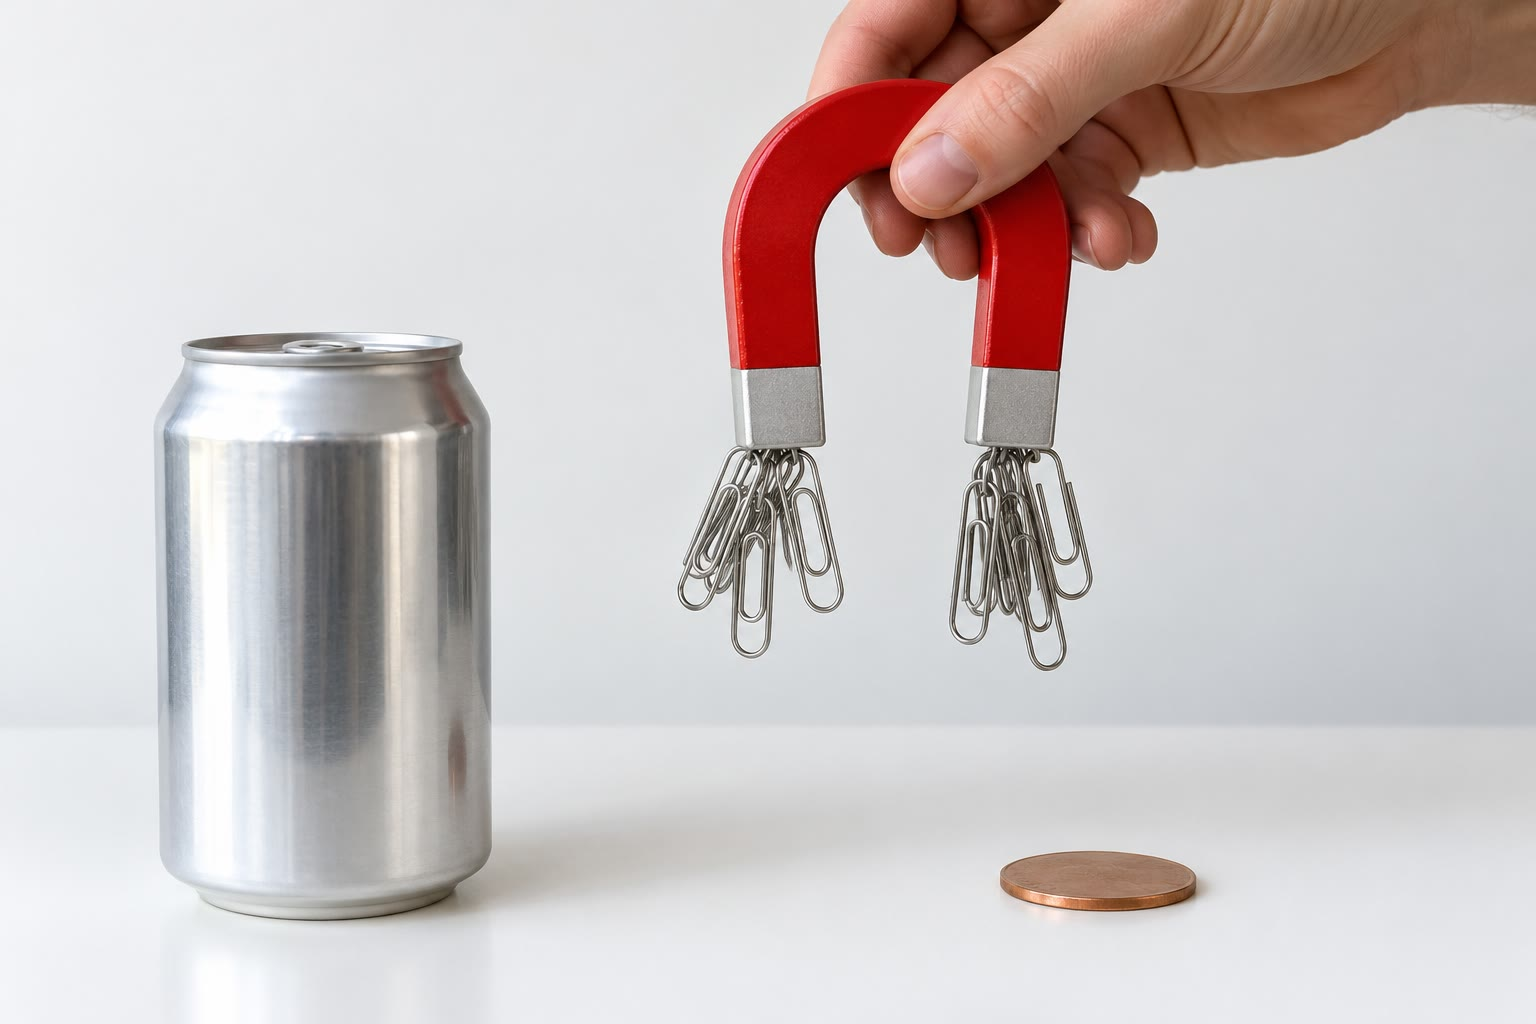
\includegraphics[width=0.55\linewidth]{images/book1/ai/g1-magnet-clips.jpg}

{\small مغناطيس يرفع مشابك ورق من الفولاذ. أما علبة الألومنيوم وقرص
النحاس على الطاولة فيبقيان في مكانهما.}
\end{omfigure}

\begin{example}[الطفو والغوص]\label{ex:g1:materials-around-us:float}
ضع بعض الأجسام في حوض ماء. قطعة الخشب وغطاء القارورة البلاستيكي
يطفوان. أما الحصاة وكرة الزجاج الصغيرة والمسمار الفولاذي فتغوص إلى
القاع. وطفو الشيء أو غوصه هو أيضًا خاصية من خصائص مادته.
\end{example}

\begin{omfigure}
\begin{tikzpicture}[font=\small]
  % the basin
  \fill[omWater!80] (0,0) rectangle (9,2.2);
  \draw[omGlass, line width=0.8pt] (-0.1,2.7) -- (0,2.6) -- (0,0) -- (9,0)
    -- (9,2.6) -- (9.1,2.7);
  % floating: wooden block, plastic cap
  \fill[brown!55, draw=brown!70!black] (0.8,2.0) rectangle (2.2,2.5);
  \fill[red!70, draw=red!50!black] (3.7,2.05) rectangle (4.3,2.35);
  % sunk: pebble, marble, nail
  \fill[black!35, draw=black!60] (5.0,0.25) ellipse (0.45 and 0.22);
  \shade[ball color=cyan!40] (6.5,0.2) circle (0.18);
  \fill[black!55] (7.6,0.06) rectangle (8.6,0.14);
  \fill[black!55] (7.52,0.02) rectangle (7.62,0.18);
  % labels
  \node[anchor=south] at (1.5,2.75) {قطعة خشب};
  \node[anchor=south] at (4.0,2.75) {غطاء بلاستيكي};
  \node[anchor=north] at (5.0,-0.1) {حصاة};
  \node[anchor=north] at (6.5,-0.1) {كرة زجاج};
  \node[anchor=north] at (8.1,-0.1) {مسمار};
  \node[anchor=west, align=left] at (9.3,2.2) {هذه تطفو};
  \node[anchor=west, align=left] at (9.3,0.2) {هذه تغوص};
\end{tikzpicture}

{\small في حوض الماء: قطعة الخشب والغطاء البلاستيكي يطفوان؛ والحصاة
وكرة الزجاج والمسمار الفولاذي تغوص.}
\end{omfigure}

\section{فرز المواد}

\begin{method}[الفرز بخاصية واحدة]\label{met:g1:materials-around-us:sort}
لفرز كومة من الأجسام:
\begin{enumerate}
  \item اختر سؤالًا \textbf{واحدًا}، مثلًا: «أيجذبه
        المغناطيس؟»؛
  \item اختبر كل \omterm{def:g1:materials-around-us:object}{جسم} وضعه في مجموعة «نعم» أو في مجموعة
        «لا»؛
  \item ثم افرز كل مجموعة من جديد بسؤال آخر إن شئت.
\end{enumerate}
سؤال واحد في كل مرة: هكذا يكون لكل \omterm{def:g1:materials-around-us:object}{جسم} مكان واحد فقط.
\end{method}

\begin{omfigure}
\begin{tikzpicture}[font=\small]
  \draw[omDef, line width=1pt] (0,0) circle (2.3);
  \draw[omProp, line width=1pt] (2.4,0) circle (2.3);
  \node[omDef, font=\small\bfseries] at (-0.6,2.65) {مصنوع من معدن};
  \node[omProp, font=\small\bfseries] at (3.0,2.65) {يجذبه المغناطيس};
  \node[font=\footnotesize] at (-1.1,0.35) {علبة مشروب};
  \node[font=\footnotesize] at (-1.1,-0.35) {سلك نحاس};
  \node[font=\footnotesize] at (1.2,0.6) {مسمار فولاذ};
  \node[font=\footnotesize] at (1.2,0) {مفتاح حديد};
  \node[font=\footnotesize] at (1.2,-0.6) {مشبك ورق};
  \node[font=\footnotesize] at (3.5,0) {(لا شيء)};
  \node[anchor=west] at (5.2,0.9) {ملعقة خشب};
  \node[anchor=west] at (5.2,0.3) {كرة زجاج};
  \node[anchor=west] at (5.2,-0.3) {وشاح صوف};
  \node[anchor=west] at (5.2,-0.9) {حصاة};
\end{tikzpicture}

{\small سؤالان وحلقتان. داخل الحلقة الزرقاء: الأجسام المصنوعة من
المعدن. داخل الحلقة البرتقالية: الأجسام التي يجذبها المغناطيس. في
الحلقتين معًا: أجسام الحديد أو الفولاذ. وخارجهما: كل ما عدا ذلك.}
\end{omfigure}

\begin{center}
\small
\begin{tabular}{lccc}
\hline
\omterm{def:g1:materials-around-us:object}{الجسم} (\omterm{def:g1:materials-around-us:material}{المادة}) & صلب؟ & شفاف؟ & يجذبه المغناطيس؟ \\
\hline
قطعة (خشب) & نعم & لا & لا \\
مسمار (فولاذ) & نعم & لا & نعم \\
كرة صغيرة (زجاج) & نعم & نعم & لا \\
غطاء قارورة (بلاستيك) & نعم & لا & لا \\
ورقة (ورق) & لا & لا & لا \\
وشاح (صوف) & لا & لا & لا \\
حصاة (حجر) & نعم & لا & لا \\
\hline
\end{tabular}
\end{center}

\section{المادة المناسبة للعمل المطلوب}

\begin{proposition}[تُختار كل مادة لخصائصها]\label{prop:g1:materials-around-us:choose}
يختار الناس \omterm{def:g1:materials-around-us:material}{مادة} \omterm{def:g1:materials-around-us:object}{الجسم} بحسب ما يجب أن يؤديه \omterm{def:g1:materials-around-us:object}{الجسم}:
\begin{itemize}
  \item يجب أن تُدخل النافذة الضوء: فهي مصنوعة من الزجاج، وهو
        شفاف؛
  \item يجب أن يمنع معطف المطر الماء وأن يُطوى: فهو مصنوع من
        البلاستيك أو من قماش لا ينفذ منه الماء؛
  \item يجب ألا يذوب القدر فوق الموقد: فهو مصنوع من المعدن؛
  \item يجب ألا تحرق يد القدر اليد: فكثيرًا ما تُصنع من الخشب
        أو من بلاستيك صلب، فهما لا يسخنان كما يسخن المعدن؛
  \item يجب أن تكون الوسادة لينة: فهي مصنوعة من قماش محشو بالريش
        أو بالألياف.
\end{itemize}
\end{proposition}

\begin{example}[القارب]\label{ex:g1:materials-around-us:boat}
يجب أن يطفو قارب اللعب. يمكن أن يُصنع من الخشب أو من البلاستيك. أما
قارب مصنوع من كتلة مصمتة من الحجر فيغوص فورًا.
\end{example}

\begin{remark}[الزجاج المكسور]\label{rem:g1:materials-around-us:glass}
الزجاج صلب لكنه ينكسر، وقطعه حادة. وإذا انكسر كأس فإن شخصًا بالغًا
هو الذي يجمع القطع.
\end{remark}

\section{تمارين}

\begin{exercise}[$\star$]\label{exo:g1:materials-around-us:1}
هل الكرسي \omterm{def:g1:materials-around-us:object}{جسم} أم \omterm{def:g1:materials-around-us:material}{مادة}؟ وهل الخشب \omterm{def:g1:materials-around-us:object}{جسم} أم \omterm{def:g1:materials-around-us:material}{مادة}؟
\end{exercise}

\begin{exercise}[$\star$]\label{exo:g1:materials-around-us:2}
سمِّ \omterm{def:g1:materials-around-us:material}{مادة} كل \omterm{def:g1:materials-around-us:object}{جسم}: لوح زجاج النافذة، والمسمار، والحصاة، والكتاب،
والجورب.
\end{exercise}

\begin{exercise}[$\star$]\label{exo:g1:materials-around-us:3}
أعطِ جسمين مصنوعين من الخشب وجسمين مصنوعين من البلاستيك.
\end{exercise}

\begin{exercise}[$\star$]\label{exo:g1:materials-around-us:4}
جد الدخيل وقل لماذا: ملعقة خشبية، وشوكة معدنية، وملعقة بلاستيكية،
وكرسي خشبي. (انظر إلى المواد.)
\end{exercise}

\begin{exercise}[$\star$]\label{exo:g1:materials-around-us:5}
أي \omterm{def:g1:materials-around-us:material}{مادة} نرى من خلالها: الخشب أم الزجاج أم الحجر؟
\end{exercise}

\begin{exercise}[$\star$]\label{exo:g1:materials-around-us:6}
نقرّب مغناطيسًا من مسمار فولاذي وكرة زجاج صغيرة وقطعة خشب. أيها
يجذب؟
\end{exercise}

\begin{exercise}[$\star$]\label{exo:g1:materials-around-us:7}
انظر إلى الشكل الذي فيه الحوض. كم جسمًا يطفو؟ وكم جسمًا
يغوص؟
\end{exercise}

\begin{exercise}[$\star$]\label{exo:g1:materials-around-us:8}
للمقص شفرتان ومقبضان. من أي \omterm{def:g1:materials-around-us:material}{مادة} صُنع كل جزء؟ وهل المقص مصنوع
من \omterm{def:g1:materials-around-us:material}{مادة} واحدة أم من مادتين؟
\end{exercise}

\begin{exercise}[$\star$]\label{exo:g1:materials-around-us:9}
انظر إلى الشكل الذي فيه الحلقتان. في أي حلقة توجد علبة المشروب؟
ولماذا ليست في الحلقة البرتقالية؟
\end{exercise}

\begin{exercise}[$\star\star$]\label{exo:g1:materials-around-us:10}
لماذا تُصنع النوافذ من الزجاج لا من الخشب؟
\end{exercise}

\begin{exercise}[$\star\star$]\label{exo:g1:materials-around-us:11}
يريد سام أن يفرز هذه الأجسام الثمانية بالسؤال «أيجذبه
المغناطيس؟»: مسمار فولاذي، ومشبك ورق، وحصاة، وملعقة خشبية، ومفتاح
حديد، وعلبة مشروب، وكرة زجاج صغيرة، وجورب صوفي. كم جسمًا يدخل
مجموعة «نعم»؟ وكم جسمًا يدخل مجموعة «لا»؟
\end{exercise}
